%\section{Event selection}
\section{Data and Monte Carlo samples}
\subsection{Data samples}

The full Run-2 dataset containing all proton-proton collision data collected from 2015-2018 at $\sqrt{s}=13$TeV with a $25$ns bunch spacing configuration are used.

In 2015, 2016, 2017, and 2018 $3.86$~fb$^{-1}$, $35.6$~fb$^{-1}$, $46.9$~fb$^{-1}$, and  $62.2$~fb$^{-1}$ of luminosity were recorded respectively. Peak instantaneous luminosity increased from $5.0\times 10^{33}$~cm$^{-2}$s$^{-1}$ in 2015 to $21.4\times 10^{33}$~cm$^{-2}$s$^{-1}$ in 2018. Average and peak pile-up also increased from about $\langle\mu\rangle=13.6$ and 40.5 in 2015 to  $\langle\mu\rangle=37.0$ and 90 in 2018. These pile-up distributions datasets are shown in \ref{fig:mu_profile}. 

\begin{figure}[!htbp]
    \centering 
    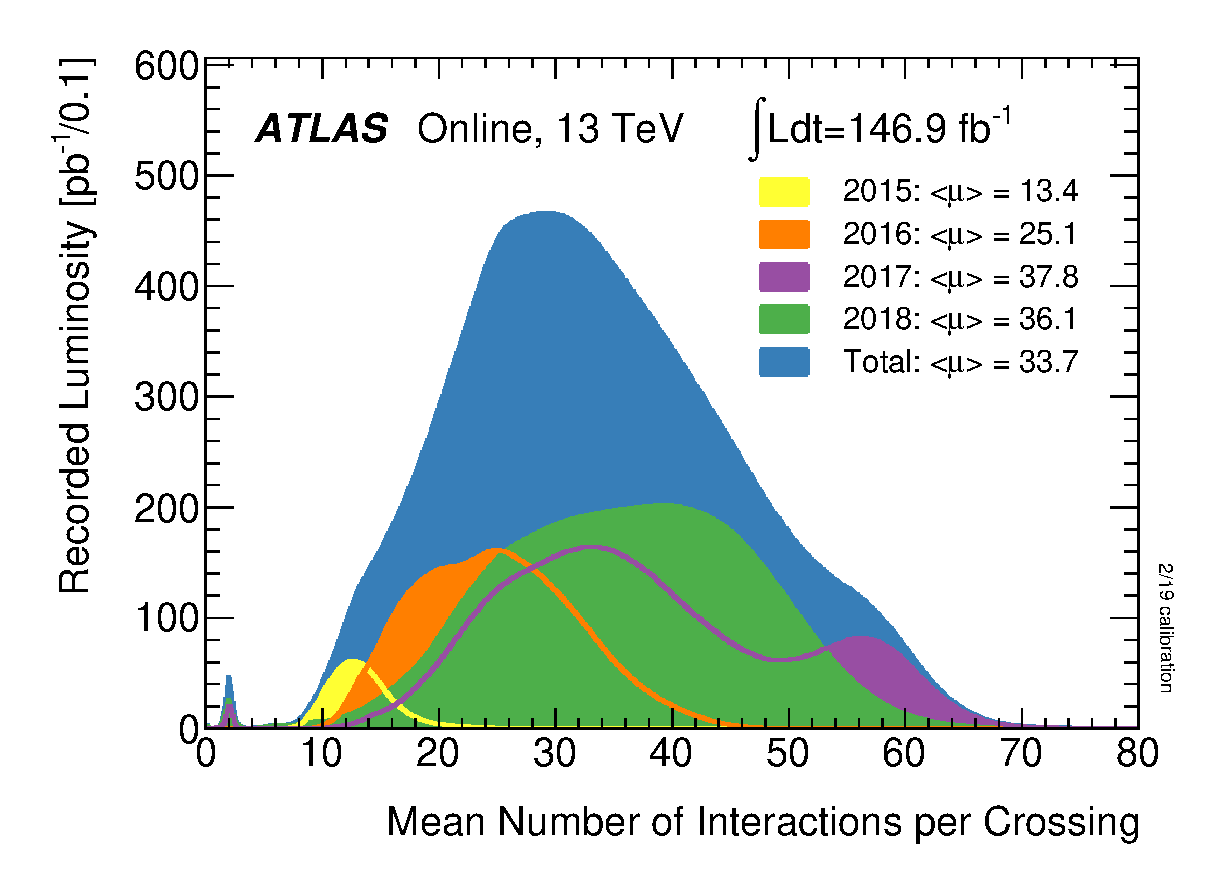
\includegraphics[width=0.55\linewidth]{Pictures/mu_2015_2018.eps}
    \caption{The luminosity-weighted distribution of the mean number of interactions per crossing is shown for Run-2 pp collision data. }
    \label{fig:mu_profile}
\end{figure}

Events are only used if all relevant detector components are operating normally. These events are part of the standard ``All Good'' Good Run List comprising a rotal integrated luminosity of $139$fb$^{-1}$ and data quality efficiency of $91.5$\%.

Throughout Run-2 the instaneous luminosity and so pile-up changed dramatically. This is accounted for in our MC modeliing, as described in the next section

%%%%%%%%%%%%%%%%%%%%%%%%%%%%%%%%%%%%
\subsection{Monte Carlo samples}

%This analysis uses samples reconstructed using release 21.0.  Derivations of MC samples were produced with the tags \texttt{p3654}, \texttt{p3652} which use \texttt{AthDerivation 21.2.44}.
%Derivations of data samples were made the tag \texttt{p3653} using \texttt{AthDerivation 21.2.44}. The samples are further processed  using \texttt{AnalysisBase 21.2.68} for systematic computation.

%\textcolor{red}{Add alternative MC samples for signal and backgrounds}\\

Monte Carlo samples are generated to compare to data in order to test Standard Model predictions and search for excesses. These simulations are also used to optimize the analysis before applying these techniques to our dataset. Monte Carlo events are fully simulated using the ATLAS detector simulation in the GEANT4 framework \cite{GEANT4} and reconstructed with standard ATLAS reconstruction software. Pile-up is simulated as additional $pp$ interations in a separate simulation step during digitization where minimum bias events are superimposted on the simulated signal events. These additional events are added based on the that years recorded pile-up to account for dataset differences. 

Separate programs are used to generate the hard scattering process and to model the parton showering (PS), hadronization, and the underlying event (UE). Different versions of \textsc{Pythia} are used for parton showering (PS), hadronisation and the underlying event (UE) depending on the MC process \cite{pythia8}. These are summarized in the following subsections which detail the simulation techniques for our signal vector boson fusion samples, other Higgs production modes, and relevant backgrounds.   

%\HERWIG~\cite{herwig} is used for PS and hadronisation in estimating systematic uncertainties with UE being modelled with \JIMMY~\cite{jimmy}.

%The CT10 and NNPDF3.0 parton distributions function (PDF) sets~\cite{Lai:2010vv}~\textcolor{red}{[missing NNPDF3.0 ref]} are used for the hard scattering process in \textsc{ Powheg-Box} v2~\cite{Nason:2009ai} ~\textcolor{red}{[unclear sinec 2 PDF sets are listed, are they used in different processes?]} while for \MADGRAPH5 (version 2.2.1 and 2.2.2)~\cite{Alwall:2014hca} the NNPDF23LO~\cite{Ball:2012cx} PDF set is used.
%The AZNLO~\cite{Aad:2014xaa} tune is used for the diboson and signal processes while the A14 tune~\cite{ATL-PHYS-PUB-2014-021} for other processes.
%The CTEQ6L1~\cite{Nadolsky:2008zw} PDF set is used for the \PYTHIA8 showering,
%with the NNPDF 3.0tune when interfaced to \textsc{ Powheg-Box} v2 and
%with the A14~\cite{ATL-PHYS-PUB-2014-021} tune when interfaced to \MADGRAPH5.

%The hard scattering NLO predictions from \SHERPA 2.2.1~\cite{Gleisberg:2008ta} are calculated using NNPDF 3.0 NNLO PDF set in conjunction with a dedicated set of tuned parameters from the parton shower developed by the \SHERPA authors~\cite{Schumann:2007mg}.

%The complete list of the MC samples and their configuration can be found in Appendix \ref{sec:append_samples}.
The fullset of data is split into three time-based categories. Data-taking conditions in 2015 and 2016 are averaged and described together as mc16a. 2017 and 2018 data-taking conditions are considered separately as mc16d and mc16e respectively. 

%%%%%%%%%%%%%%%%%%%%%%%%%%%%%%%%%%%%%%%%%%%%%%%%%%%%%%
\subsubsection{Vector boson fusion Higgs samples}

VBF Higgs events are generated through \textsc{POWHEG} \cite{Nason:2009ai} interfaced with \textsc{Pythia} 8 with the PDF4LHC15 parton distribution function (PDF) set \cite{PDF4LHC15}. Cross sections are calculated with full NLO QCD and EW corrections \cite{CiccoliniDennerDittmaier2007,Arnold2009} with an approximate NNLO QCD correction applied~\cite{Bolzoni2010}. These cross-sections as well as associated branching ratios are calculated by the LHC Higgs Cross Section Working Group Yellow Report 4 \cite{deFlorian:2016spz}. Generated events are normalized to calculated cross-sections. Two tables below show first the production cross sections used to normalize the Higgs MC samples (including those for VBF) \ref{tab:MCSignal} and next summaries of the MC samples used including nominal production as well as alternative productions for the estimation of theoretical systematics, which are discussed further in the next chapter \ref{tab:samples}.  
%%%%%%%%%%%%%%%%%%%%%%%%%%%%%%%%%%%%%%%%%%%%%%%%%%%%%%
\subsubsection{Other production mode Higgs samples}

\begin{table*}[tb]
 \centering
 \caption{SM Higgs boson production cross sections ($\sigma$) for gluon fusion, vector-boson fusion and associated production with a $W$ or $Z$ boson or with a $b\bar{b}$ or $t\bar{t}$ pair in $pp$ collisions at $\sqrt{s}=13$ TeV. First and second uncertainties represent theoretical systematic uncertainties calculated by adding in quadrature the QCD scale and PDF$+\alpha_s$ uncertainties, respectively. The last column shows the decay branching ratio ($B$) for $H \rightarrow \ell\nu\ell\nu$ with $\ell = e, \mu$.\label{tab:MCSignal}}
 \vspace{0.1cm}
 \begin{tabular}{ccccccc}
   \hline \hline
   \noalign{\vspace{0.05cm}}
   $m_{H}$       & $\sigma\left(gg\to H\right)$ & $\sigma\left(qq'\to Hqq'\right)$ & $\sigma\left(q\bar{q}\to WH\right)$ & $\sigma\left(pp\to ZH\right)$   \\
   $[{\GeV}]$ & $[{\textrm{pb}}]$                 & $[{\textrm{pb}}]$                     &  $[{\textrm{pb}}]$                       & $[{\textrm{pb}}]$                    \\
   \noalign{\vspace{0.05cm}}
   \hline\hline
   \noalign{\vspace{0.05cm}}
% TODO: take the gaussian errors instead of flat for ggF N3LO as recommended?
   
   $125.0$\rule[-1mm]{0mm}{4.7mm} & $48.58$  $^{+4.6\%}_{-6.7\%}$ $^{+3.2\%}_{-3.2\%}$ & $3.782$  $^{+0.4\%}_{-0.3\%}$ $^{+2.1\%}_{-2.1\%}$ & $1.373$  $^{+0.5\%}_{-0.7\%}$ $^{+1.9\%}_{-1.9\%}$  
                                  & $0.8839$ $^{+3.8\%}_{-3.1\%}$ $^{+1.6\%}_{-1.6\%}$ \\
  
   \noalign{\vspace{0.05cm}}
   \hline\hline 
   \noalign{\vspace{0.05cm}}
   $m_{H}$       & $\sigma\left(gg\to ZH\right)$ & $\sigma\left(q\bar{q}/gg\to t\bar{t}H\right)$ & $\sigma\left(q\bar{q}/gg\to b\bar{b}H\right)$ & $B$ (\htollllbrief)   \\ 
   $[{\GeV}]$ & $[{\textrm{pb}}]$                  & $[{\textrm{pb}}]$                                  & $[{\textrm{pb}}]$                                 & $[10^{-3}]$\\
   \noalign{\vspace{0.05cm}}
   \hline\hline
   \noalign{\vspace{0.05cm}}
    $125.0$\rule[-1mm]{0mm}{4.7mm} & $0.1227$ $^{+25.1\%}_{-18.9\%}$ $^{+2.4\%}_{-2.4\%}$ & $0.5071$ $^{+5.8\%}_{-9.2\%}$ $^{+3.6\%}_{-3.6\%}$ & $0.4880$ $^{+20.2\%}_{-23.9\%}$ & $0.1240$ $\pm2.18\%$ \\
   \noalign{\vspace{0.05cm}}
   \hline\hline
 \end{tabular}
\end{table*}  

Other Higgs production modes gluon fusion (ggF), associated Higgs boson production ($VH$, $V=W,Z$) and Higgs boson production in association with a heavy quark pair ($ttH$, $bbH$) are important backgrounds din this analysis and listed in table \ref{tab:samples}. ggF and $ttH$ production samples are also produced using \textsc{Madgraph5$_$aMC@NLO} for cross-checks. \textcolor{red}{Check the Madgraph and add other VBF?} 

Similar to the VBF Higgs sample, ggF, $VH$, $ttH$ and $bbH$ are produced with \textsc{Pythia8}\cite{pythia,Sjostrand:2007gs} for decay, parton shower, hadronisation and multiple parton interactions.

\begin{table}[tb]
\caption{MC samples used to simulate Higgs boson production, including generators, QCD calculation accuracy and PDF sets.}
\label{tab:samples}
\centering
\begin{tabular}{ llll}
  \hline
  \hline
  Process & Generator & Accuracy in QCD & PDF set   \\
  \hline
   VBF & \progname{Powheg-Box} v2~\cite{powheg1,powheg2,powheg3,powheg5}  & NLO & PDF4LHC~\cite{Butterworth:2015oua} \\
 \hline 
  ggF & \progname{Powheg-Box} v2 (NNLOPS)~\cite{powheg1,powheg2,powheg3,Campbell:2012am} & NNLO in $y^{H}$~\cite{Hamilton:2013fea}, & PDF4LHC~\cite{Butterworth:2015oua}  \\
  & & $p_{T}^{H}$ consistent with \progname{HqT}  & \\
  & & (NNLO+NNLL)~\cite{Bozzi:2005wk,deFlorian:2011xf} & \\  
  $VH$ & \progname{Powheg-Box} v2 (\progname{MiNLO})~\cite{powheg1,powheg2,powheg3,Luisoni:2013kna} & NLO & PDF4LHC~\cite{Butterworth:2015oua} \\
  $tH$ & \progname{Powheg-Pythia8} & NLO & PDF4LHC~\cite{Butterworth:2015oua} \\
  $\ttH$ & \progname{Powheg-Box} v2~\cite{powheg1,powheg2,powheg3,powheg5} & NLO & PDF4LHC~\cite{Butterworth:2015oua} \\
  $bbH$ & \progname{Madgraph5\_aMC@NLO} (v.2.3.3)~\cite{Alwall:2014hca,Wiesemann:2014ioa} & NLO & NNPDF23~\cite{Ball:2012cx} \\
\hline
\hline
\end{tabular}
\end{table}
 
%%%%%%%%%%%%%%%%%%%%%%%%%%%%%%%%%%%%%%%
\subsubsection{Background samples}
\label{sec:bkgMC}

\begin{table}[h]
  \centering
  \caption{MC generators used to model the signal and background processes, and corresponding cross sections.  When the leptonic decay filter is applied on $W/Z$ bosons the quoted cross sections include the branching ratios and are summed over lepton flavors. The column ``Precision $\sigma_{\mathrm{incl.}}$'' gives the precision of the inclusive cross section applied to the sample. Precise MC generator versions and details of the generator level cuts are given in the text.}
%  \scalebox{0.75}{
{\footnotesize
  \begin{tabular}{llrcc}
    \hline\hline
    Process & Generator & \hspace*{-3mm}$\sigma\cdot\mathrm{Br}$ (pb) & Precision $\sigma_{\mathrm{incl.}}$\\
\hline 
%VBF $H\rightarrow WW$  & \POWHEG+\PythiaEight & 0.808 & NNLO \\
%    \hline
%%    ggF $H\rightarrow WW $  & \POWHEG+\PythiaEight & 10.4 & NNLO+NNLL \\
%    ggF $H\rightarrow WW $  & \POWHEG NNLOPS & 10.4 & NNLO+NNLL \\
%    $WH$ $H\rightarrow WW $ & \POWHEG+\PythiaEight (MINLO) & 0.293  & NNLO \\ % TO  BE checked
%    $ZH$ $H\rightarrow WW $ & \POWHEG+\PythiaEight (MINLO) & 0.189  & NNLO \\ % TO  BE checked
%   \red{ttH, tH, and bbH}
    \hline 
    \hline
    $q\bar{q}/g\rightarrow WW \rightarrow \ell\nu\ell\nu$              & \SHERPA 2.2.2 & 49.74  & NLO\\ 
    $Z^{(\ast)}Z^{(\ast)} \to 2\ell2\nu~(m_{\ell\ell} \ge 4 \gev)$     & \SHERPA  2.1  & 6.53   & NLO\\

    $gg \to  2\ell2\nu$                     & \SHERPA  2.1 & 0.87 & NLO\\

    $q\bar{q}/g \to  \ell\nu\ell\ell$       & \SHERPA 2.1 & 11.9 & NLO\\

    $q\bar{q}/g, gg \to  \ell\ell\ell\ell$  & \SHERPA 2.1 & 11.5 & NLO\\


    EW $WW + 2$ jets $(\ell\nu\ell\nu)$   & \SHERPA 2.1 & 0.012 & LO \\
    EW $WZ + 2$ jets $(\ell\nu\ell\ell)$  & \SHERPA 2.1 & 0.038 & LO \\
    EW $ZZ + 2$ jets $(\ell\ell\ell\ell)$ & \SHERPA 2.1 & 0.116 & LO \\
    EW $q\bar{q} {\to}(Z\rightarrow\tau\tau) q\bar{q}$ & \SHERPA & 2.54 & LO\\
    \hline
     inclusive $Z/\gamma^{\star} \to \ell\ell~(40 \ge m_{\ell\ell} \ge 10 \gev)$ & \SHERPA 2.2.1 & $6.80 \times 10^{3}$ & NNLO\\ %%UPdate XS
    inclusive $Z/\gamma^{\star} \to \ell\ell~( m_{\ell\ell} \ge 40 \gev)$       & \SHERPA 2.2.1 & $2.107 \times 10^{3}$ & NNLO\\

    $(W \to \ell\nu)\gamma~(p_{T}^{\gamma} > 7 \gev)$                 & \SHERPA 2.2.2& 453 & NLO\\
    $(Z \to \ell\ell)\gamma~(p_{T}^{\gamma} > 7 \gev)$                & \SHERPA 2.2.2& 175 & NLO\\

    $\ttbar$ di-leptonic($e,\mu ,\tau$)         & \PythiaEight & 87.6 & NNLO+NNLL & \\
    $Wt$ leptonic             & \POWHEG+\PythiaSix & 7.55 &  NLO & \\
     \hline\hline
  \end{tabular}
  }
  \label{tab:mcsamples}
\end{table}

The main sources of SM backgrounds include events from the production of dibosons, top-quark, $Z$+jets, $W$+jets and multijets. They are summarised in Tab.~\ref{tab:mcsamples}.

The $WW$ samples are generated using \SHERPA 2.2.2 interfaced with NNPDF3.0 NNLO PDFs, as described in Ref.~\cite{Cascioli:2013gfa}.
The samples is generated with 0 and 1 jet at NLO accuracy and 2 and 3 jet at LO accuracy.
The following requirements are used for the production: $\mll>4$ GeV, $\pT(l1)>5$ GeV, $\pT(l2)>5$ GeV. 
The loop-induced $gg$-initiated diboson processes are simulated by \SHERPA 2.1.1 with zero or one additional jets, as described in Ref.~\cite{Cascioli:2013gfa}.
In case of $WW$, the sample is normalized to the NLO $gg\rightarrow WW$ cross section calculated in Ref.~\cite{Caola:2015rqy} at $\rts=13~\tev$. Thus, a k-factor of 2.3 \textcolor{red}{AT: are we sure it is 2.3? I remember 1.6} is applied to the sample.
%AT: For all other processes the cross sections are taken from the generator and are at LO. 

For $q\bar{q}/g{\to}Z^{(\ast)}Z^{(\ast)}{\to}\ell\nu\ell\nu$ by $\POWHEG$ v2 a cut on the
invariant mass of the two charged lepton $m_{\ell\ell} > 4 ~\gev$ is required, here $m_{\ell}$ is the mass of the charged lepton, for any same-flavour opposite-sign (SFOS) lepton pairs.
In addition it is required that at least two charged leptons must have $\pT > 5 ~\gev$.
The $ZZ$ is also simulated with \SHERPA 2.1, as alternative sample.

The $WZ$ is generated with \SHERPA 2.1, using the CT10 PDFs, at NLO accurary for 0 and 1 jet and LO for 2 and 3.
These samples include also the $\gamma*$ process and are produced with the following cut:
$\mll>2 \times m_{l}+250$ MeV, $\pT(l1)>5$ GeV, $\pT(l2)>5$ GeV.

%The $ZZ$ is also simulated with \SHERPA 2.1.
%For the $W$+jets estimation, which will be described in Section~\ref{sec:FakeEstimation}, 
%all the diboson process, except for $gg\to ZZ$, are simulated with \POWHEG+\PythiaEight.

%Diboson samples are generated using \SHERPA 2.2.1 interfaced with NNPDF 3.0 NNLO PDFs and normalised to cross sections calculated at NLO\cite{CampbellEllis2010}.
%%%% EW samples  
The \SHERPA 2.1.1 MC is used for the modeling of diboson process with no $O(\alpha_S)$ terms for the $\ell\ell\ell\ell, \ell\nu\ell\ell$ and $\ell\nu\ell\nu$ plus two jets final states as well as the $q\bar{q}{\to}Zq\bar{q}$ processes with a requirement of $Z{\to}\tau\tau$ ($m_{\tau\tau} > 40 \gev$) decay,
which are also known as electroweak (EW) processes, at the LO accuracy.

$Z$+jets (also referred to as DY) production is simulated with \SHERPA 2.2.1 using the NNPDF3.0 NNLO PDFs with dedicated parton shower tuning developed by the Sherpa authors. 
In order to generate sufficient high V ($\pT$) statistics, V+jets samples are split according to max($H_T$, $p_T^V$). 
Additionally, to obtain sufficient heavy-flavour final state statistics, the V+jets samples are generated applying filters.
Moreover, for the $Z \to \tau \tau$ an additional filter on the leptons( or hadrons) $\pT$ has been added to better populate the analysis phase space.
Five filtered regions have been defined, but only 2 are used in $\hwwlnln$: lep13lep7, lep15had20.
Only the first three max($H_T$, $p_T^V$) slices are available with these filters.
Therefore, in the $\hwwlnln$ up to $140<$max($H_T$, $p_T^V$)$<280$ the lepton/had $\pT$ filtered samples are used instead for the high max($H_T$, $p_T^V$) slice the nominal samples are used.
Samples are normalised using cross sections calculated at NNLO accuracy~\cite{MelnikovPetriello}.

The top-quark pair production is also simulated using \POWHEG with the \textsc{ Powheg-Box} framework using the NNPDF 3.0 PDFs and interfaced with \PythiaEight using NNPDF 2.3 PDFs for parton showering, with A14 tune.
The $t\bar{t}$ samples generated include a filter to require that the $W$ bosons decays leptonically. All the three leptons ($e, \mu, \tau$) are considered for the $W$ decay in \POWHEG. The $\tau$s are then decayed by \PythiaEight in either leptonically or hadronically mode.
Samples are normalised using cross sections calculated at NNLO+NNLL~\cite{Czakon:2013}.

The single top, mainly $Wt$, production is generated with
\textsc{Powheg-Box}\,2.0 interfaced to \PYTHIA 6.428 for parton showering, using \textsc{Perugia}2012~\cite{Skands:2010ak} tune.
\textsc{ EvtGen}\,1.2.0~\cite{Lange:2001uf} is used for properties of the bottom and charm hadron decays.
%The predicted $\ttbar$ production cross section is calculated with the \textsc{Top++2.0}
%program to NNLO in perturbative QCD, including soft-gluon resummation to 
%NNLL order (see~\cite{Czakon:2011xx} and references therein), and assuming a top-quark mass of 172.5 $\gev$.
$Wt$ sample is required to have at least two charged leptons in the final state.
%Both $\ttbar$ and $Wt$ samples are required to have at least two charged leptons in the final state.

$Z\gamma$ and $W\gamma$ productions are modeled using \SHERPA 2.2.2 at the NLO accuracy for 0- and 1-jet.
For both $Z\gamma$ and $W\gamma$ processes the $\pt$ of the $\gamma$ are
required to be larger than 7 $\gev$, and the distance in the $\eta - \phi$ plane
$\Delta R = \sqrt{(\Delta \eta)^{2} + (\Delta \phi)^{2}} > 0.1$.
In addition the leptons from $Z$ boson in the $Z\gamma$ final state is required to have $m_{\ell\ell} > 2 \gev$.

The $W$+jets process modeling is based on a purely data-driven method described in Sect.~\ref{sec:FakeEstimation}.
However, MC samples are used to validate the fake estimation as well as to estimate the sample composition uncertainties, see Section~\ref{sec:FakeEstimation}. For those studies, same MC generators are used to predict the $W$+jets and $Z$+jets.
The $V$+jets processes are generated with \POWHEG MiNLO interfaced to \PythiaEight with the AZNLO tune. 
The PDF set used in \POWHEG is CT14nnlo whereas the PDF set used in the parton shower is the CTEQ6 L1 leading order set.
The alternative V+jets samples have been produced using the LO matrix-element generator ALPGEN v2.14 interfaced to \PythiaSix to model the parton shower. The parton-shower tune Perugia2011C and the CTEQ6L1 PDF set have been used. 
Up to five additional partons are modelled by the matrix elements, merged with the MLM prescription with a matching scale of 20 GeV. 
The predictions follow a four-flavour-number-scheme (4FNS) for the production of heavy-flavour jets.
%Other MC generators, like \SHERPA and \MadGraph, are availble h
%AT All simulated samples include the effect of pile-up from multiple interactions in the same and neighbouring bunch crossing. 
%AT This is achieved by overlaying minimum bias events, simulated using \PythiaEight, using A2 tune and interfaced with MSTW2008LO PDFs. 
%AT All samples are processed through the Geant-4 based ATLAS detector simulation, and reconstructed with the standard ATLAS reconstruction software

\section{Object definitions}
\section{Event selection}
